\documentclass{ximera}

%% You can put user macros here
%% However, you cannot make new environments

\listfiles

\graphicspath{{./}{firstExample/}{secondExample/}}

\usepackage{tikz}
\usepackage{tkz-euclide}
\usepackage{tikz-3dplot}
\usepackage{tikz-cd}
\usetikzlibrary{shapes.geometric}
\usetikzlibrary{arrows}
\usetikzlibrary{decorations.pathmorphing,patterns}
\usetkzobj{all}
\pgfplotsset{compat=1.13} % prevents compile error.

\renewcommand{\vec}[1]{\mathbf{#1}}
\newcommand{\RR}{\mathbb{R}}
\newcommand{\dfn}{\textit}
\newcommand{\dotp}{\cdot}
\newcommand{\id}{\text{id}}
\newcommand\norm[1]{\left\lVert#1\right\rVert}
 
\newtheorem{general}{Generalization}
\newtheorem{initprob}{Exploration Problem}

\tikzstyle geometryDiagrams=[ultra thick,color=blue!50!black]

\usepackage{mathtools}
%\input{../../../../fimacros.tex}



\title{Nonhomogeneous Linear Equations}


\begin{document}

\begin{abstract}

\end{abstract}

\maketitle

\section*{Nonhomogeneous Linear Equations}

We'll now consider the nonhomogeneous linear second order equation
\begin{equation} \label{eq:5.3.1}
y''+p(x)y'+q(x)y=f(x),
\end{equation}
where the forcing function $f$ isn't  identically zero. The next
theorem, an extension of Theorem~\ref{thmtype:5.1.1}, gives sufficient
conditions for existence and uniqueness of solutions of initial value
problems for \eqref{eq:5.3.1}. We omit the proof, which is beyond the
scope of this book.

\begin{theorem}\label{thmtype:5.3.1}
Suppose $p$, $q$ and $f$ are continuous on an open interval
$(a,b)$, let $x_0$ be any point in $(a,b)$, and let $k_0$ and $k_1$ be
arbitrary real numbers. Then the initial value problem
$$
y''+p(x)y'+q(x)y=f(x), \quad  y(x_0)=k_0,\quad y'(x_0)=k_1
$$
 has a unique solution  on $(a,b)$.
\end{theorem}

To find the general solution of  \eqref{eq:5.3.1}
on an interval $(a,b)$ where $p$, $q$, and $f$ are continuous,
it's necessary to find the general solution  of
 the associated homogeneous equation
\begin{equation} \label{eq:5.3.2}
y''+p(x)y'+q(x)y=0
\end{equation}
on $(a,b)$. We call \eqref{eq:5.3.2} the \textit{complementary equation}
for \eqref{eq:5.3.1}.

The next theorem shows how to find the general solution of
\eqref{eq:5.3.1} if we know one solution $y_p$ of \eqref{eq:5.3.1} and a
fundamental set of solutions of \eqref{eq:5.3.2}. We call
$y_p$ a \textit{particular solution} of \eqref{eq:5.3.1};   it
can be any solution that we can find,  one way or another.

\begin{theorem}\label{thmtype:5.3.2}
Suppose $p$, $q$, and $f$ are continuous on $(a,b)$. Let $y_p$
be a particular solution of
\begin{equation} \label{eq:5.3.3}
y''+p(x)y'+q(x)y=f(x)
\end{equation}
on $(a,b)$, and let  $\{y_1,y_2\}$ be a fundamental set of solutions
of the complementary equation
\begin{equation} \label{eq:5.3.4}
y''+p(x)y'+q(x)y=0
\end{equation}
on $(a,b)$.
Then $y$ is a solution of  $\eqref{eq:5.3.3}$ on $(a,b)$ if and  only if
\begin{equation} \label{eq:5.3.5}
y=y_p+c_1y_1+c_2y_2,
\end{equation}
where $c_1$ and $c_2$  are constants.
\end{theorem}

\begin{proof} We first show that $y$ in \eqref{eq:5.3.5} is a solution of
\eqref{eq:5.3.3} for any choice of the constants $c_1$ and $c_2$.
Differentiating \eqref{eq:5.3.5} twice yields
$$
y'=y_p'+c_1y_1'+c_2y_2'\quad\mbox{and}\quad
y''=y_p''+ c_1y_1''+c_2y_2'',
$$
so
\begin{eqnarray*}
y''+p(x)y'+q(x)y&=&(y_p''+c_1y_1''+c_2y_2'')
+p(x)(y_p'+c_1y_1'+c_2y_2')\\&&\; +q(x)(y_p+c_1y_1+c_2y_2)\\
&=&(y_p''+p(x)y_p'+q(x)y_p)+c_1(y_1''+p(x)y_1'+q(x)y_1)\\
&&\; +c_2(y_2''+p(x)y_2'+q(x)y_2)\\
&=& f+c_1\cdot0+c_2\cdot 0=f,
\end{eqnarray*}
since $y_p$ satisfies \eqref{eq:5.3.3} and $y_1$ and $y_2$ satisfy
\eqref{eq:5.3.4}.

Now we'll show that every solution of \eqref{eq:5.3.3} has the form
\eqref{eq:5.3.5} for some choice of the constants $c_1$ and  $c_2$.
Suppose $y$ is a solution of \eqref{eq:5.3.3}. We'll show that
$y-y_p$ is a solution of \eqref{eq:5.3.4}, and therefore of the form
$y-y_p=c_1y_1+c_2y_2$, which implies \eqref{eq:5.3.5}. To see this, we
compute
\begin{eqnarray*}
(y-y_p)''+p(x)(y-y_p)'+q(x)(y-y_p)&=&(y''-y_p'')+p(x)(y'-y_p')\\ &&
+q(x)(y-y_p)\\
&=&(y''+p(x)y'+q(x)y)\\ && -(y_p''+p(x)y_p'+q(x)y_p)\\
&=&f(x)-f(x)=0,
\end{eqnarray*}
since $y$ and $y_p$ both satisfy \eqref{eq:5.3.3}. 
\end{proof}

We say that \eqref{eq:5.3.5} is the \dfn{general solution of
$\eqref{eq:5.3.3}$ on $(a,b)$}.


If $P_0$, $P_1$, and $F$ are continuous and $P_0$ has no zeros on
$(a,b)$, then  Theorem~\ref{thmtype:5.3.2} implies that the general
solution of
\begin{equation} \label{eq:5.3.6}
P_0(x)y''+P_1(x)y'+P_2(x)y=F(x)
\end{equation}
on  $(a,b)$ is $y=y_p+c_1y_1+c_2y_2$, where $y_p$ is a particular
solution  of \eqref{eq:5.3.6} on $(a,b)$ and  $\{y_1,y_2\}$ is a
fundamental set of solutions of
$$
P_0(x)y''+P_1(x)y'+P_2(x)y=0
$$
on $(a,b)$. To see this, we rewrite \eqref{eq:5.3.6} as
$$
y''+\frac{P_1(x)}{P_0(x)}y'+\frac{P_2(x)}{P_0(x)}y=\frac{F(x)}{P_0(x)}
$$
and apply Theorem~\ref{thmtype:5.3.2} with $p=P_1/P_0$, $q=P_2/P_0$, and
$f=F/P_0$.


To avoid awkward wording in examples and exercises, we won't specify
the interval $(a,b)$ when we ask for the general solution of a
specific linear second order equation, or for a fundamental set of
solutions of a homogeneous linear second order equation. Let's agree
that this always means that we want the general solution (or a
fundamental set of solutions, as the case may be) on every open
interval on which $p$, $q$, and $f$ are continuous if the equation is
of the form \eqref{eq:5.3.3}, or on which $P_0$, $P_1$, $P_2$, and $F$ are
continuous and $P_0$ has no zeros, if the equation is of the form
\eqref{eq:5.3.6}. We leave it to you to identify these intervals in
specific examples and exercises.

For completeness, we point out that if $P_0$, $P_1$, $P_2$, and $F$ are
all continuous on an open interval $(a,b)$, but $P_0$  does
have a zero in $(a,b)$, then \eqref{eq:5.3.6} may fail to have a general
solution on $(a,b)$ in the sense just defined.
% Exercises~\ref{exer:5.1.42}--\ref{exer:5.1.44}
%illustrate this point for a homogeneous equation.

In this section we to limit ourselves to applications of
Theorem~\ref{thmtype:5.3.2} where we can guess at the form of the
particular solution.

\begin{example}\label{example:5.3.1} 
\begin{enumerate}
\item \label{item:5.3.1a} % (a)
Find the general solution of
\begin{equation} \label{eq:5.3.7}
y''+y=1.
\end{equation}
\item \label{item:5.3.1b} % (b)
Solve the initial value problem
\begin{equation} \label{eq:5.3.8}
y''+y=1, \quad  y(0)=2,\quad y'(0)=7.
\end{equation}
\end{enumerate}


\begin{explanation} \ref{item:5.3.1a}
We can apply Theorem~\ref{thmtype:5.3.2} with $(a,b)= (-\infty,\infty)$,
since the functions $p\equiv0$, $q\equiv1$, and $f\equiv1$ in
\eqref{eq:5.3.7} are continuous on $(-\infty,\infty)$. By inspection we
see that $y_p\equiv1$ is a particular solution of \eqref{eq:5.3.7}. Since
$y_1=\cos x$ and $y_2=\sin x$ form a fundamental set of solutions of
the complementary equation $y''+y=0$, the general solution of
\eqref{eq:5.3.7} is
\begin{equation} \label{eq:5.3.9}
y=1+c_1\cos x+c_2\sin x.
\end{equation}

\ref{item:5.3.1b}
Imposing the initial condition $y(0)=2$ in \eqref{eq:5.3.9} yields
$2=1+c_1$, so $c_1=1$. Differentiating \eqref{eq:5.3.9} yields
$$
y'=-c_1\sin x+c_2\cos x.
$$
Imposing the initial condition $y'(0)=7$ here yields $c_2=7$,
so the solution of \eqref{eq:5.3.8} is
$$
y=1+\cos x+7\sin x.
$$
The figure below shows a graph of this solution.


\begin{image}
  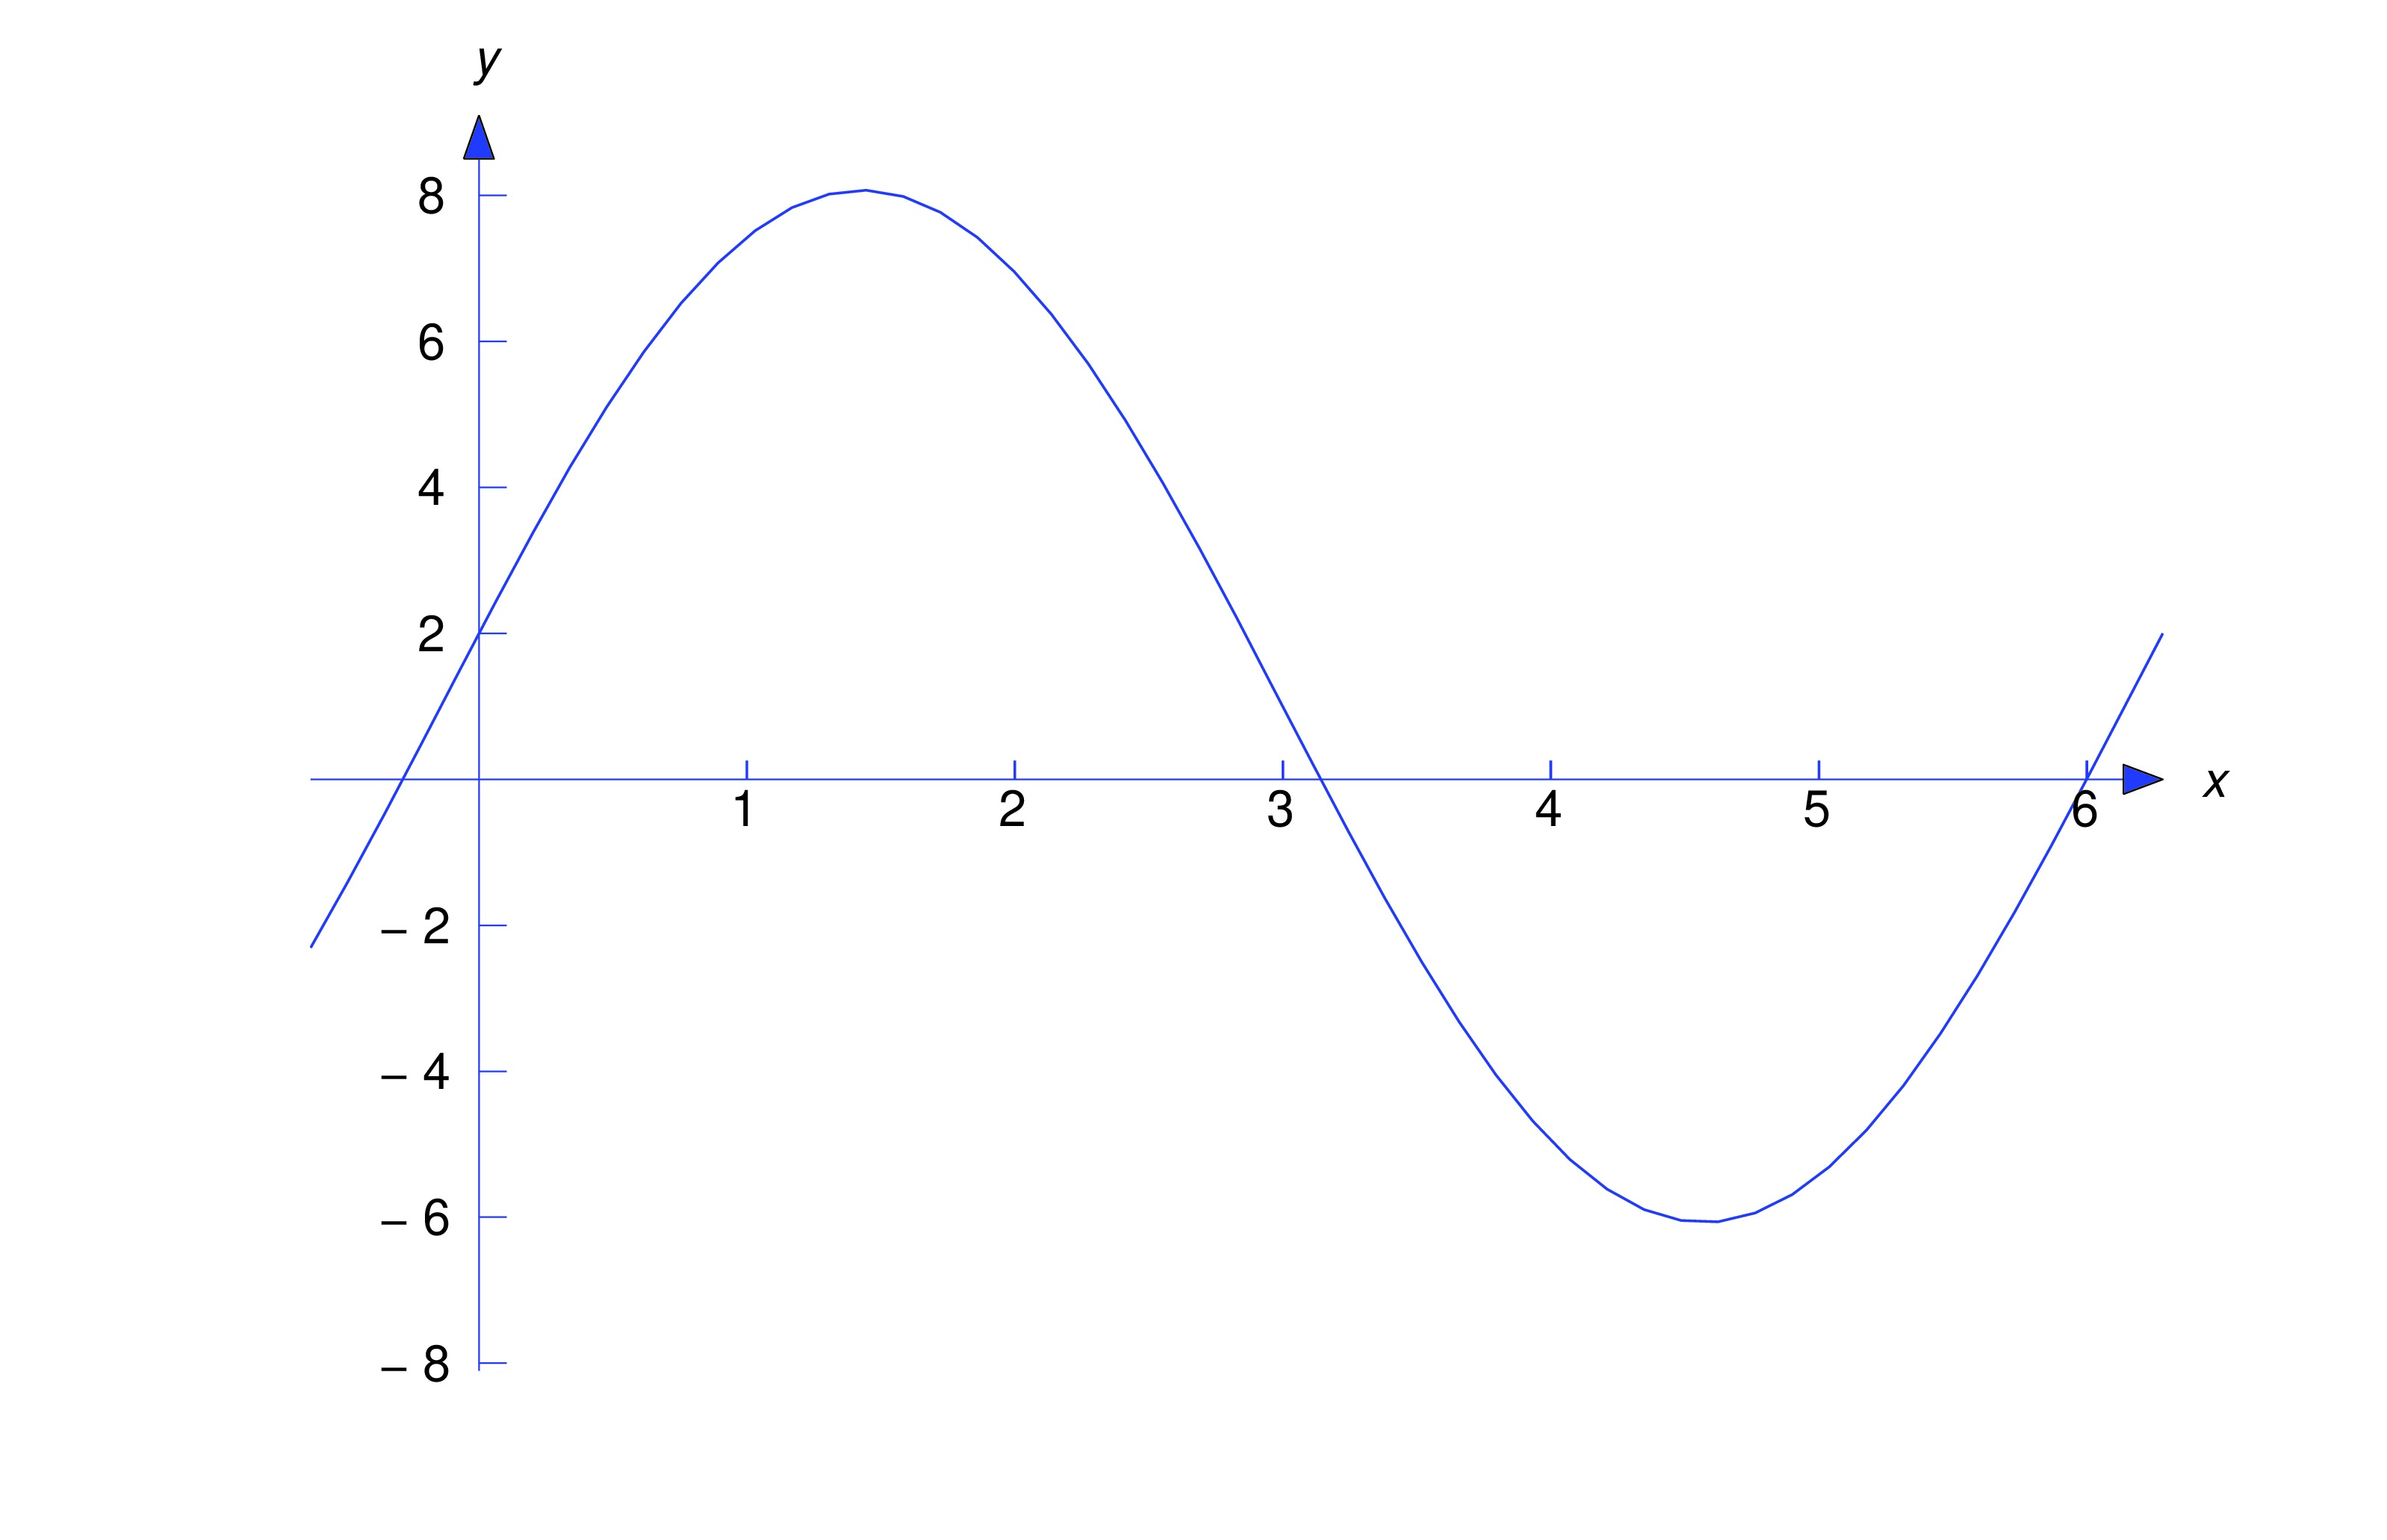
\includegraphics[height=1.5in]{fig050301.jpg} 
\end{image}

\end{explanation}
\end{example}



\begin{example}\label{example:5.3.2} 
\begin{enumerate}
\item \label{item:5.3.2a} % (a)
Find the general solution of
\begin{equation} \label{eq:5.3.10}
y''-2y'+y=-3-x+x^2.
\end{equation}
\item \label{item:5.3.2b} % (b)
Solve the initial value problem
\begin{equation} \label{eq:5.3.11}
y''-2y'+y=-3-x+x^2, \quad  y(0)=-2,\quad y'(0)=1.
\end{equation}
\end{enumerate}

\begin{explanation}
\ref{item:5.3.2a}

The characteristic polynomial of the complementary equation
$$
y''-2y'+y=0
$$
is $r^2-2r+1=(r-1)^2$,
so $y_1=e^x$ and $y_2=xe^x$  form a fundamental set of solutions
of the complementary equation. To guess  a form for a particular
solution of \eqref{eq:5.3.10}, we note that substituting a second
degree polynomial $y_p=A+Bx+Cx^2$ into the left side of \eqref{eq:5.3.10}
will produce another second degree polynomial with coefficients that
depend upon $A$, $B$, and $C$. The trick is to choose $A$, $B$, and
$C$ so the polynomials on the two sides of \eqref{eq:5.3.10} have the
same coefficients;   thus,
if
$$
y_p=A+Bx+Cx^2\quad\mbox{then}\quad
y_p'=B+2Cx\quad\mbox{and}\quad y_p''=2C,
$$
so
\begin{eqnarray*}
y_p''-2y_p'+y_p&=&2C-2(B+2Cx)+(A+Bx+Cx^2)\\
&=&(2C-2B+A)+(-4C+B)x+Cx^2=-3-x+x^2.
\end{eqnarray*}
Equating  coefficients of like powers of $x$ on the two sides of the
last equality yields
\begin{eqnarray*}
C&=&1\\
B-4C&=&-1\\
A-2B+2C&=& -3
\end{eqnarray*}
so $C=1$, $B=-1+4C=3$, and $A=-3-2C+2B=1$.
Therefore $y_p=1+3x+x^2$ is a particular solution of
\eqref{eq:5.3.10} and  Theorem~\ref{thmtype:5.3.2} implies that
\begin{equation} \label{eq:5.3.12}
y=1+3x+x^2+e^x(c_1+c_2x)
\end{equation}
is the general solution of \eqref{eq:5.3.10}.

\ref{item:5.3.2b} Imposing the initial condition $y(0)=-2$ in
\eqref{eq:5.3.12} yields $-2=1+c_1$, so $c_1=-3$. Differentiating
\eqref{eq:5.3.12} yields
$$
y'=3+2x+e^x(c_1+c_2x)+c_2e^x,
$$
and imposing the initial condition $y'(0)=1$ here yields
$1=3+c_1+c_2$, so $c_2=1$. Therefore the solution of \eqref{eq:5.3.11}
is
$$
y=1+3x+x^2-e^x(3-x).
$$
The figure below shows a graph of this solution.

\begin{image}
  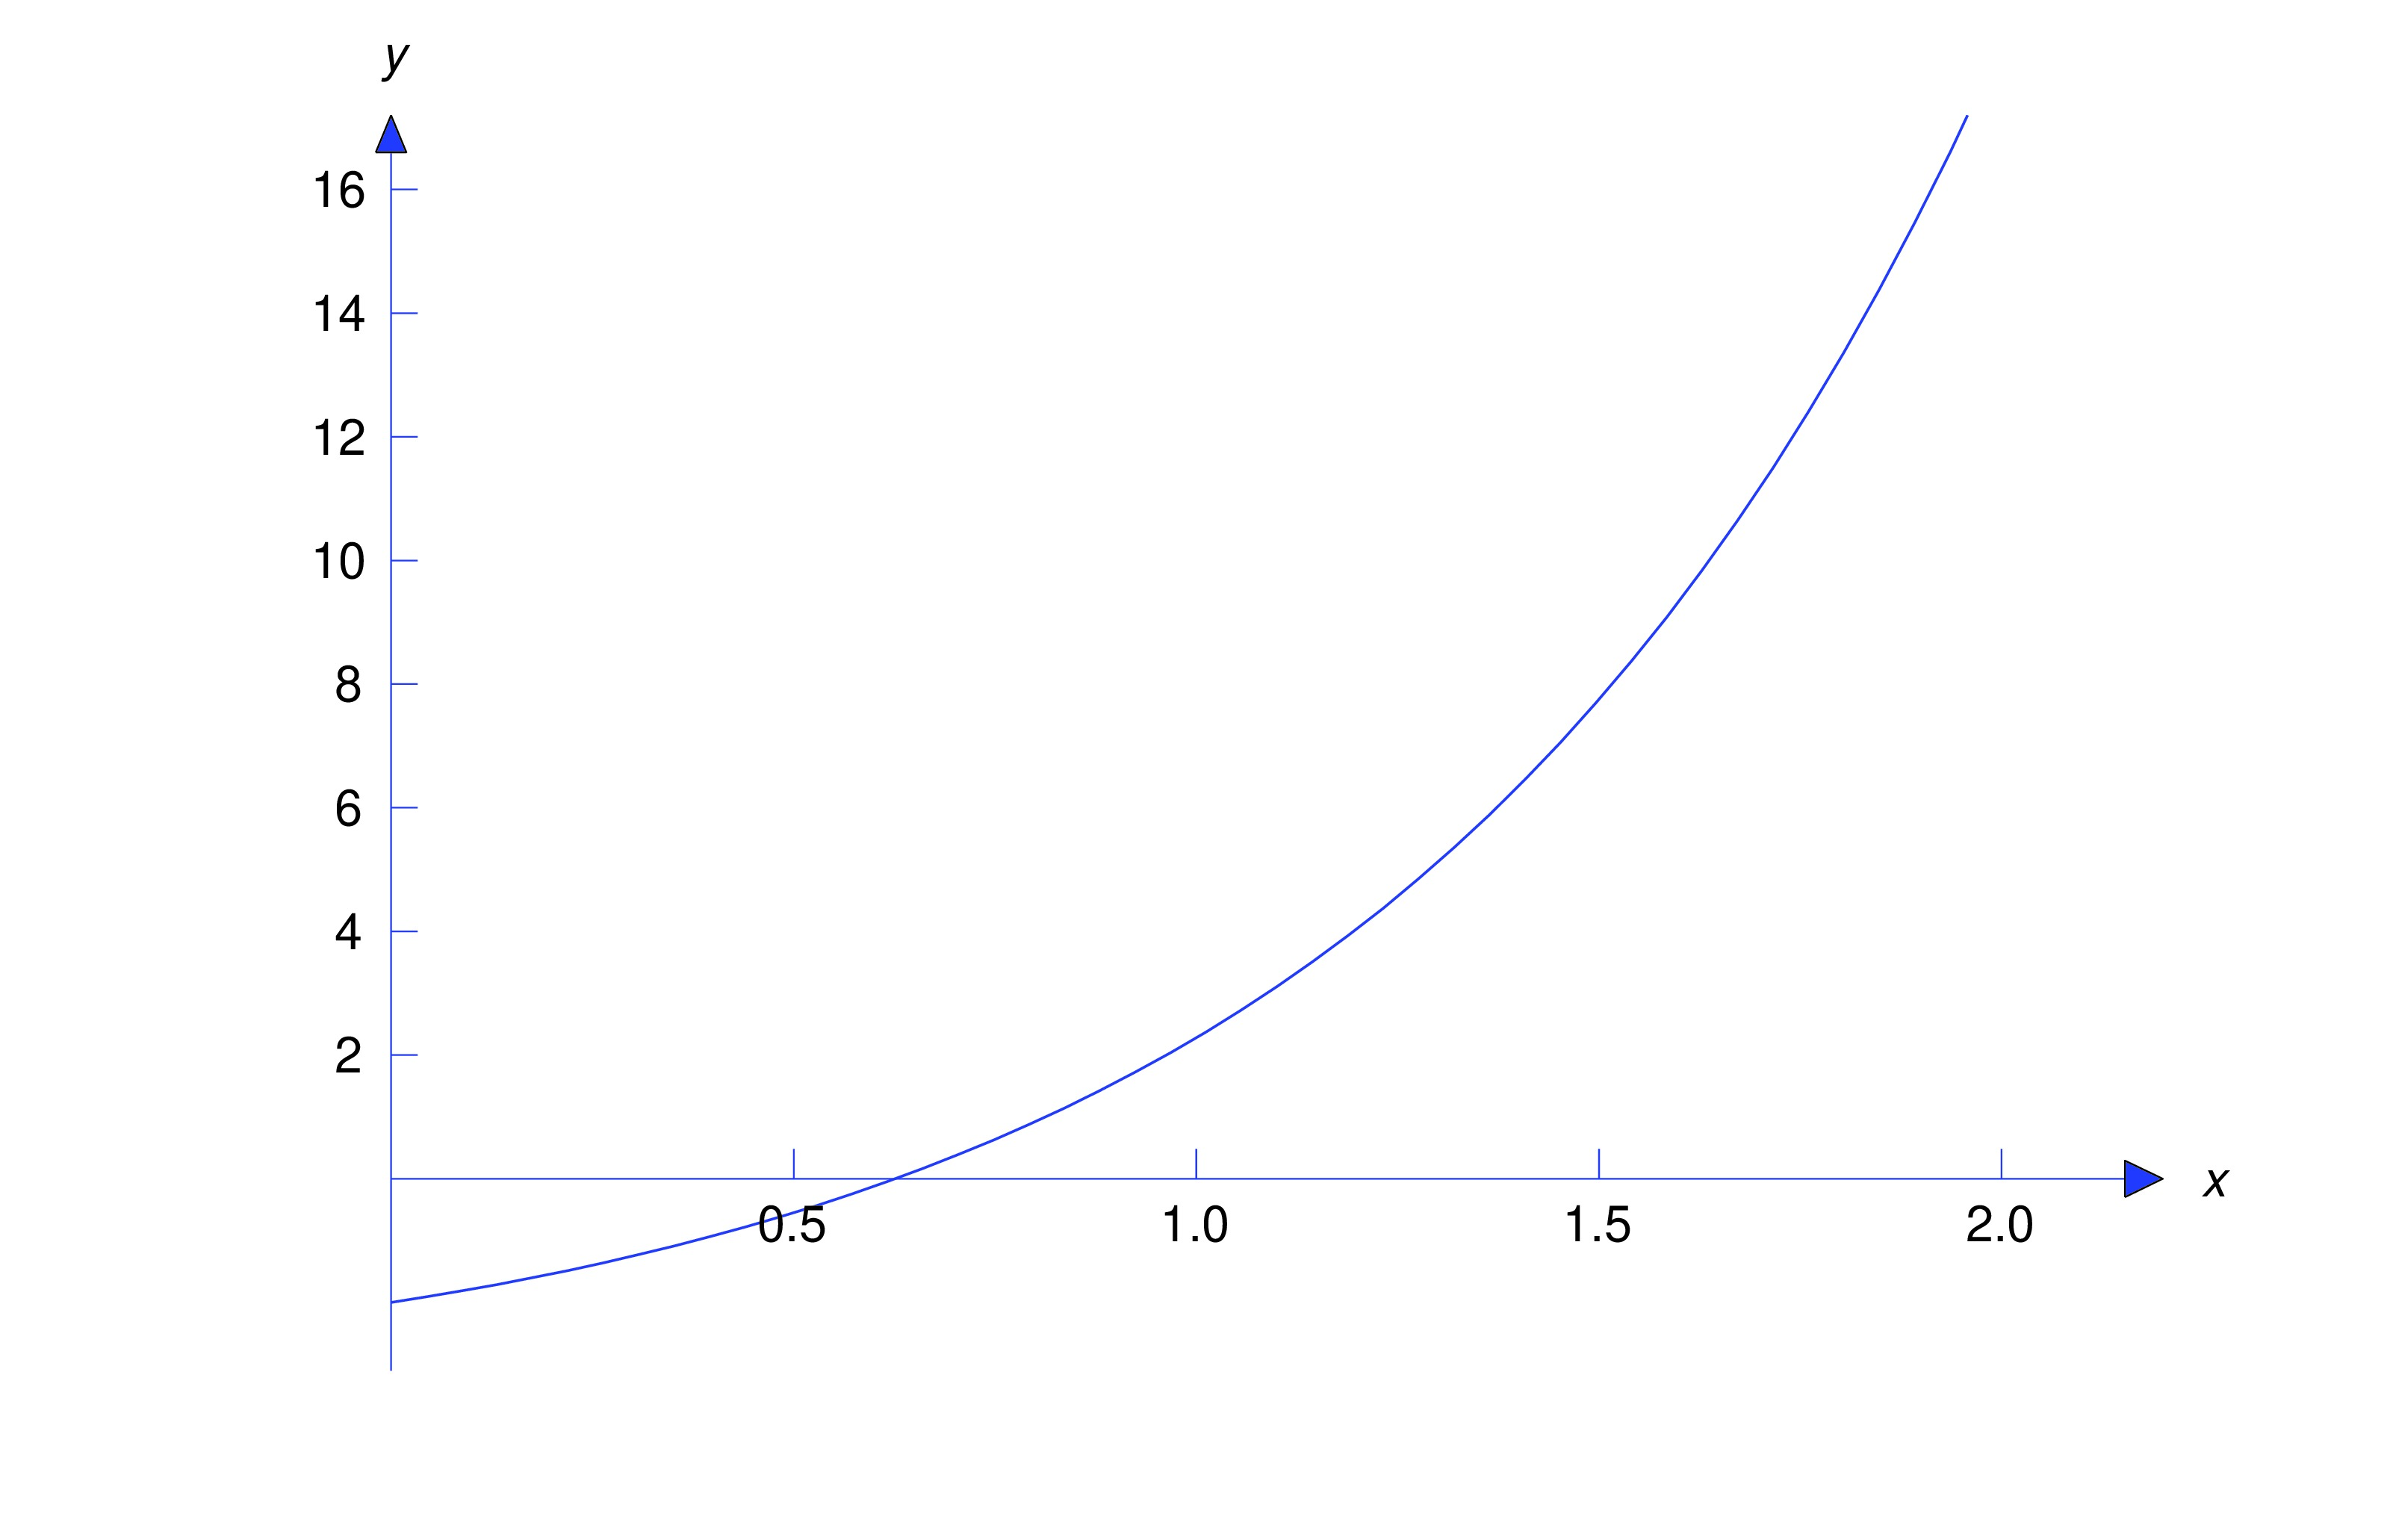
\includegraphics[height=1.5in]{fig050302.jpg} 
\end{image}

\end{explanation}
\end{example}

\begin{example}\label{example:5.3.3} 
Find the general solution of
\begin{equation} \label{eq:5.3.13}
x^2y''+xy'-4y=2x^4
\end{equation}
on $(-\infty,0)$ and $(0,\infty)$.


\begin{explanation}
In Example~\ref{example:5.1.3},  we verified that $y_1=x^2$ and $y_2=1/x^2$
form a fundamental set of solutions of the complementary equation
$$
x^2y''+xy'-4y=0
$$
on $(-\infty,0)$ and $(0,\infty)$.  To find a particular solution of
\eqref{eq:5.3.13}, we note that if
$y_p=Ax^4$, where $A$ is a constant then  both sides of \eqref{eq:5.3.13}
will be constant
multiples  of $x^4$ and  we may be able to choose  $A$ so the two sides
are equal. This is true in this example, since if $y_p=Ax^4$ then
$$
x^2y_p''+xy_p'-4y_p=x^2(12Ax^2)+x(4Ax^3)-4Ax^4=12Ax^4=2x^4
$$
if $A=1/6$;  therefore, $y_p=x^4/6$ is a particular solution of
\eqref{eq:5.3.13} on  $(-\infty,\infty)$.
Theorem~\ref{thmtype:5.3.2} implies that the general solution of
\eqref{eq:5.3.13} on  $(-\infty,0)$ and  $(0,\infty)$ is
$$
y=\frac{x^4}{6}+c_1x^2+\frac{c_2}{x^2}.
$$
\end{explanation}
\end{example}

\subsection*{The Principle of Superposition}

The next theorem enables us to break a nonhomogeous equation into
simpler parts, find a particular solution for each part, and then
combine their solutions to obtain a particular solution of the
original problem.

\begin{theorem}[The Principle of Superposition]
\label{thmtype:5.3.3} 
Suppose  $y_{p_1}$ is a particular solution of
$$
y''+p(x)y'+q(x)y=f_1(x)
$$
on $(a,b)$ and $y_{p_2}$ is a particular solution of
$$
y''+p(x)y'+q(x)y=f_2(x)
$$
on   $(a,b)$.
 Then
$$
y_p=y_{p_1}+y_{p_2}
$$
is a particular  solution of
$$
y''+p(x)y'+q(x)y=f_1(x)+f_2(x)
$$
on  $(a,b)$.
\end{theorem}

\begin{proof} If $y_p=y_{p_1}+y_{p_2}$ then
\begin{eqnarray*}
y_p''+p(x)y_p'+q(x)y_p&=&(y_{p_1}+y_{p_2})''+p(x)(y_{p_1}+y_{p_2})'
+q(x)(y_{p_1}+y_{p_2})\\
&=&\left(y_{p_1}''+p(x)y_{p_1}'+q(x)y_{p_1}\right)
+\left(y_{p_2}''+p(x)y_{p_2}'+q(x)y_{p_2}\right)\\
&=&f_1(x)+f_2(x).
\end{eqnarray*}
\end{proof}


It's easy to generalize  Theorem~\ref{thmtype:5.3.3}
to the equation
\begin{equation} \label{eq:5.3.14}
y''+p(x)y'+q(x)y=f(x)
\end{equation}
where
$$
f=f_1+f_2+\cdots+f_k;
$$
thus, if $y_{p_i}$ is a particular solution of
$$
y''+p(x)y'+q(x)y=f_i(x)
$$
on $(a,b)$ for $i=1$, $2$, \dots, $k$, then
$y_{p_1}+y_{p_2}+\cdots+y_{p_k}$
is a particular solution of \eqref{eq:5.3.14} on $(a,b)$. Moreover, by a
proof similar to the proof of Theorem~\ref{thmtype:5.3.3} we can formulate
the principle of superposition in terms of a linear equation written
in the form
$$
P_0(x)y''+P_1(x)y'+P_2(x)y=F(x)
$$
%(Exercise~\ref{exer:5.3.39});
   that is, if $y_{p_1}$
is a particular solution of
$$
P_0(x)y''+P_1(x)y'+P_2(x)y=F_1(x)
$$
on $(a,b)$ and $y_{p_2}$ is a particular solution of
$$
P_0(x)y''+P_1(x)y'+P_2(x)y=F_2(x)
$$
on  $(a,b)$, then $y_{p_1}+y_{p_2}$ is a solution of
$$
P_0(x)y''+P_1(x)y'+P_2(x)y=F_1(x)+F_2(x)
$$
on $(a,b)$.

\begin{example}\label{example:5.3.4} 
The function
 $y_{p_1}=x^4/15$ is a   particular solution of
\begin{equation} \label{eq:5.3.15}
x^2y''+4xy'+2y=2x^4
\end{equation}
on $(-\infty,\infty)$
and  $y_{p_2}=x^2/3$  is a particular solution of
\begin{equation} \label{eq:5.3.16}
x^2y''+4xy'+2y=4x^2
\end{equation}
on $(-\infty,\infty)$.
Use  the principle of superposition to
find a particular solution of
\begin{equation} \label{eq:5.3.17}
x^2y''+4xy'+2y=2x^4+4x^2
\end{equation}
on $(-\infty,\infty)$.


\begin{explanation}  The right side $F(x)=2x^4+4x^2$ in \eqref{eq:5.3.17}
is the sum of the right sides
$$
F_1(x)=2x^4\quad\mbox{and}\quad F_2(x)=4x^2.
$$
in  \eqref{eq:5.3.15}  and \eqref{eq:5.3.16}.
Therefore the principle of superposition implies that
$$
y_p=y_{p_1}+y_{p_2}=\frac{x^4}{15}+\frac{x^2}{3}
$$
is a particular solution of \eqref{eq:5.3.17}.
\end{explanation}
\end{example}

\section*{Text Source}
Trench, William F., "Elementary Differential Equations" (2013). Faculty Authored and Edited Books \& CDs. 8. (CC-BY-NC-SA)

\href{https://digitalcommons.trinity.edu/mono/8/}{https://digitalcommons.trinity.edu/mono/8/}

\end{document}


